\chapter{Design}
The focus of this paper is to explore the differences between a single model and a multistage architecture for throughput prediction in wireless networks. The choice of machine learning or deep learning model must therefore be consistent across all models considered to avoid confusing the issue with that of comparing one ML (machine learning) or DL (deep learning) method of regression with another. Lstm (long short-term memory) networks are recognised as effective models for time series forecasting \cite{8614252}, with deep learning models in general performing well in networking related tasks \cite{8666641}. As such any individual model considered in this paper is some form of Lstm deep network. Initial comparisons of multistage vs a single model ensure that all Lstm models have the same hyperparameters. That is to say, all models have the same number of nodes, layers, the same dropout chance, activation function, optimizer, etc. The only difference between the individual models considered will be that the classifier model has a different output layer to the traditional regression models as it aims to predict the class of the input sequence as opposed to the DL\_bitrate horizon. In total there are 5 individual Lstm models that had to be trained with brief description given in \ref{tab:brief_models}

\begin{table}[!htb]
  \centering
  \caption{Lstm Deep Models Used}
  \begin{tabular}{|c|c|c|}
  \hline
    {Model} & {Training Data} & {Outputs} \\
    \hline
	Baseline & All TP examples & DL\_bitrate prediction horizon \\
	\hline
	Low & Only Low TP examples & DL\_bitrate prediction horizon \\
	\hline
	Medium & Only Medium TP examples & DL\_bitrate prediction horizon \\
	\hline
	High & Only High TP examples & DL\_bitrate prediction horizon \\
	\hline
	Classifier & All labelled TP examples & Class probability table \\
  \hline
  \end{tabular}
  \label{tab:brief_models}
\end{table}


In \ref{CONSTRAINTS HEREHERHEHREHR} the number of parameters of the Lstm models were altered in various ways in order to achieve memory size parity between the single baseline throughput predictor and the multistage predictors. This is an important point to explore as adoption of a multistage approach vs a single model on mobile devices will require that both methods have comparable performance on hardware. A multistage approach could only be considered more optimal if the required memory and inference time were comparable. By design a multistage approach will be bigger than a single model, as such the total number of parameters of both approaches should be equalised for further comparison.

\section{Model Tuning}
\label{sec:model_tuning}
A hyperparameter is a parameter whose value is set before the learning process begins. In machine learning, a hyperparameter is a configuration variable that is used to control the training process, as opposed to the parameters of the model such as weights and biases, which are learned from the data. For Lstm deep models there are a number of hyperparameters than can be altered by the user, a few of note are:

- Choice of optimiser\\
- Learning rate \\
- Number of hidden nodes \\
- Number of layers \\
- Inclusion of dropout layers \\
- Dropout chance

Hyperparameter tuning is the practice of optimising the hyperparameters of a model in order to achieve better model performance. The impact of hyperparameters is wide reaching. The choice of hyperparameters not only affects the predictive performance of the model and model size, but also impacts less obvious metrics such as inference latency \cite{10.1145/3506695}. For models intended for low power devices such as mobile devices and IoT (internet of things) devices, hyperparameter tuning is even more important, as it can influence the battery consumption of the device \cite{10.1145/3506695}. The issue is with hyperparameter tuning is that the choice of hyperparameters leads to an infinite set of possible models. There are many methods for tuning deep learning models. As the models were implemented in Tensorflow, we made use of KerasTuner \cite{omalley2019kerastuner}, a tuning framework that allows for a low code solution to this issue. Random search was used to explore the possible set of combinations of hyperparameters as it is known to perform better than similar tools such as grid search \cite{bergstra2012random}. 

It must be noted that due to hardware and time limitations, only 10 such combinations of hyperparameters were considered for each model. The model was trained on each set of hyperparameters 3 times, in an attempt to account for different initialisation states leading to differences in model performance. This process was by no means extensive and given more time and computational power, a larger set of hyperparameters should be considered.

\section{Multistage One}
\begin{figure}[h]
\centering
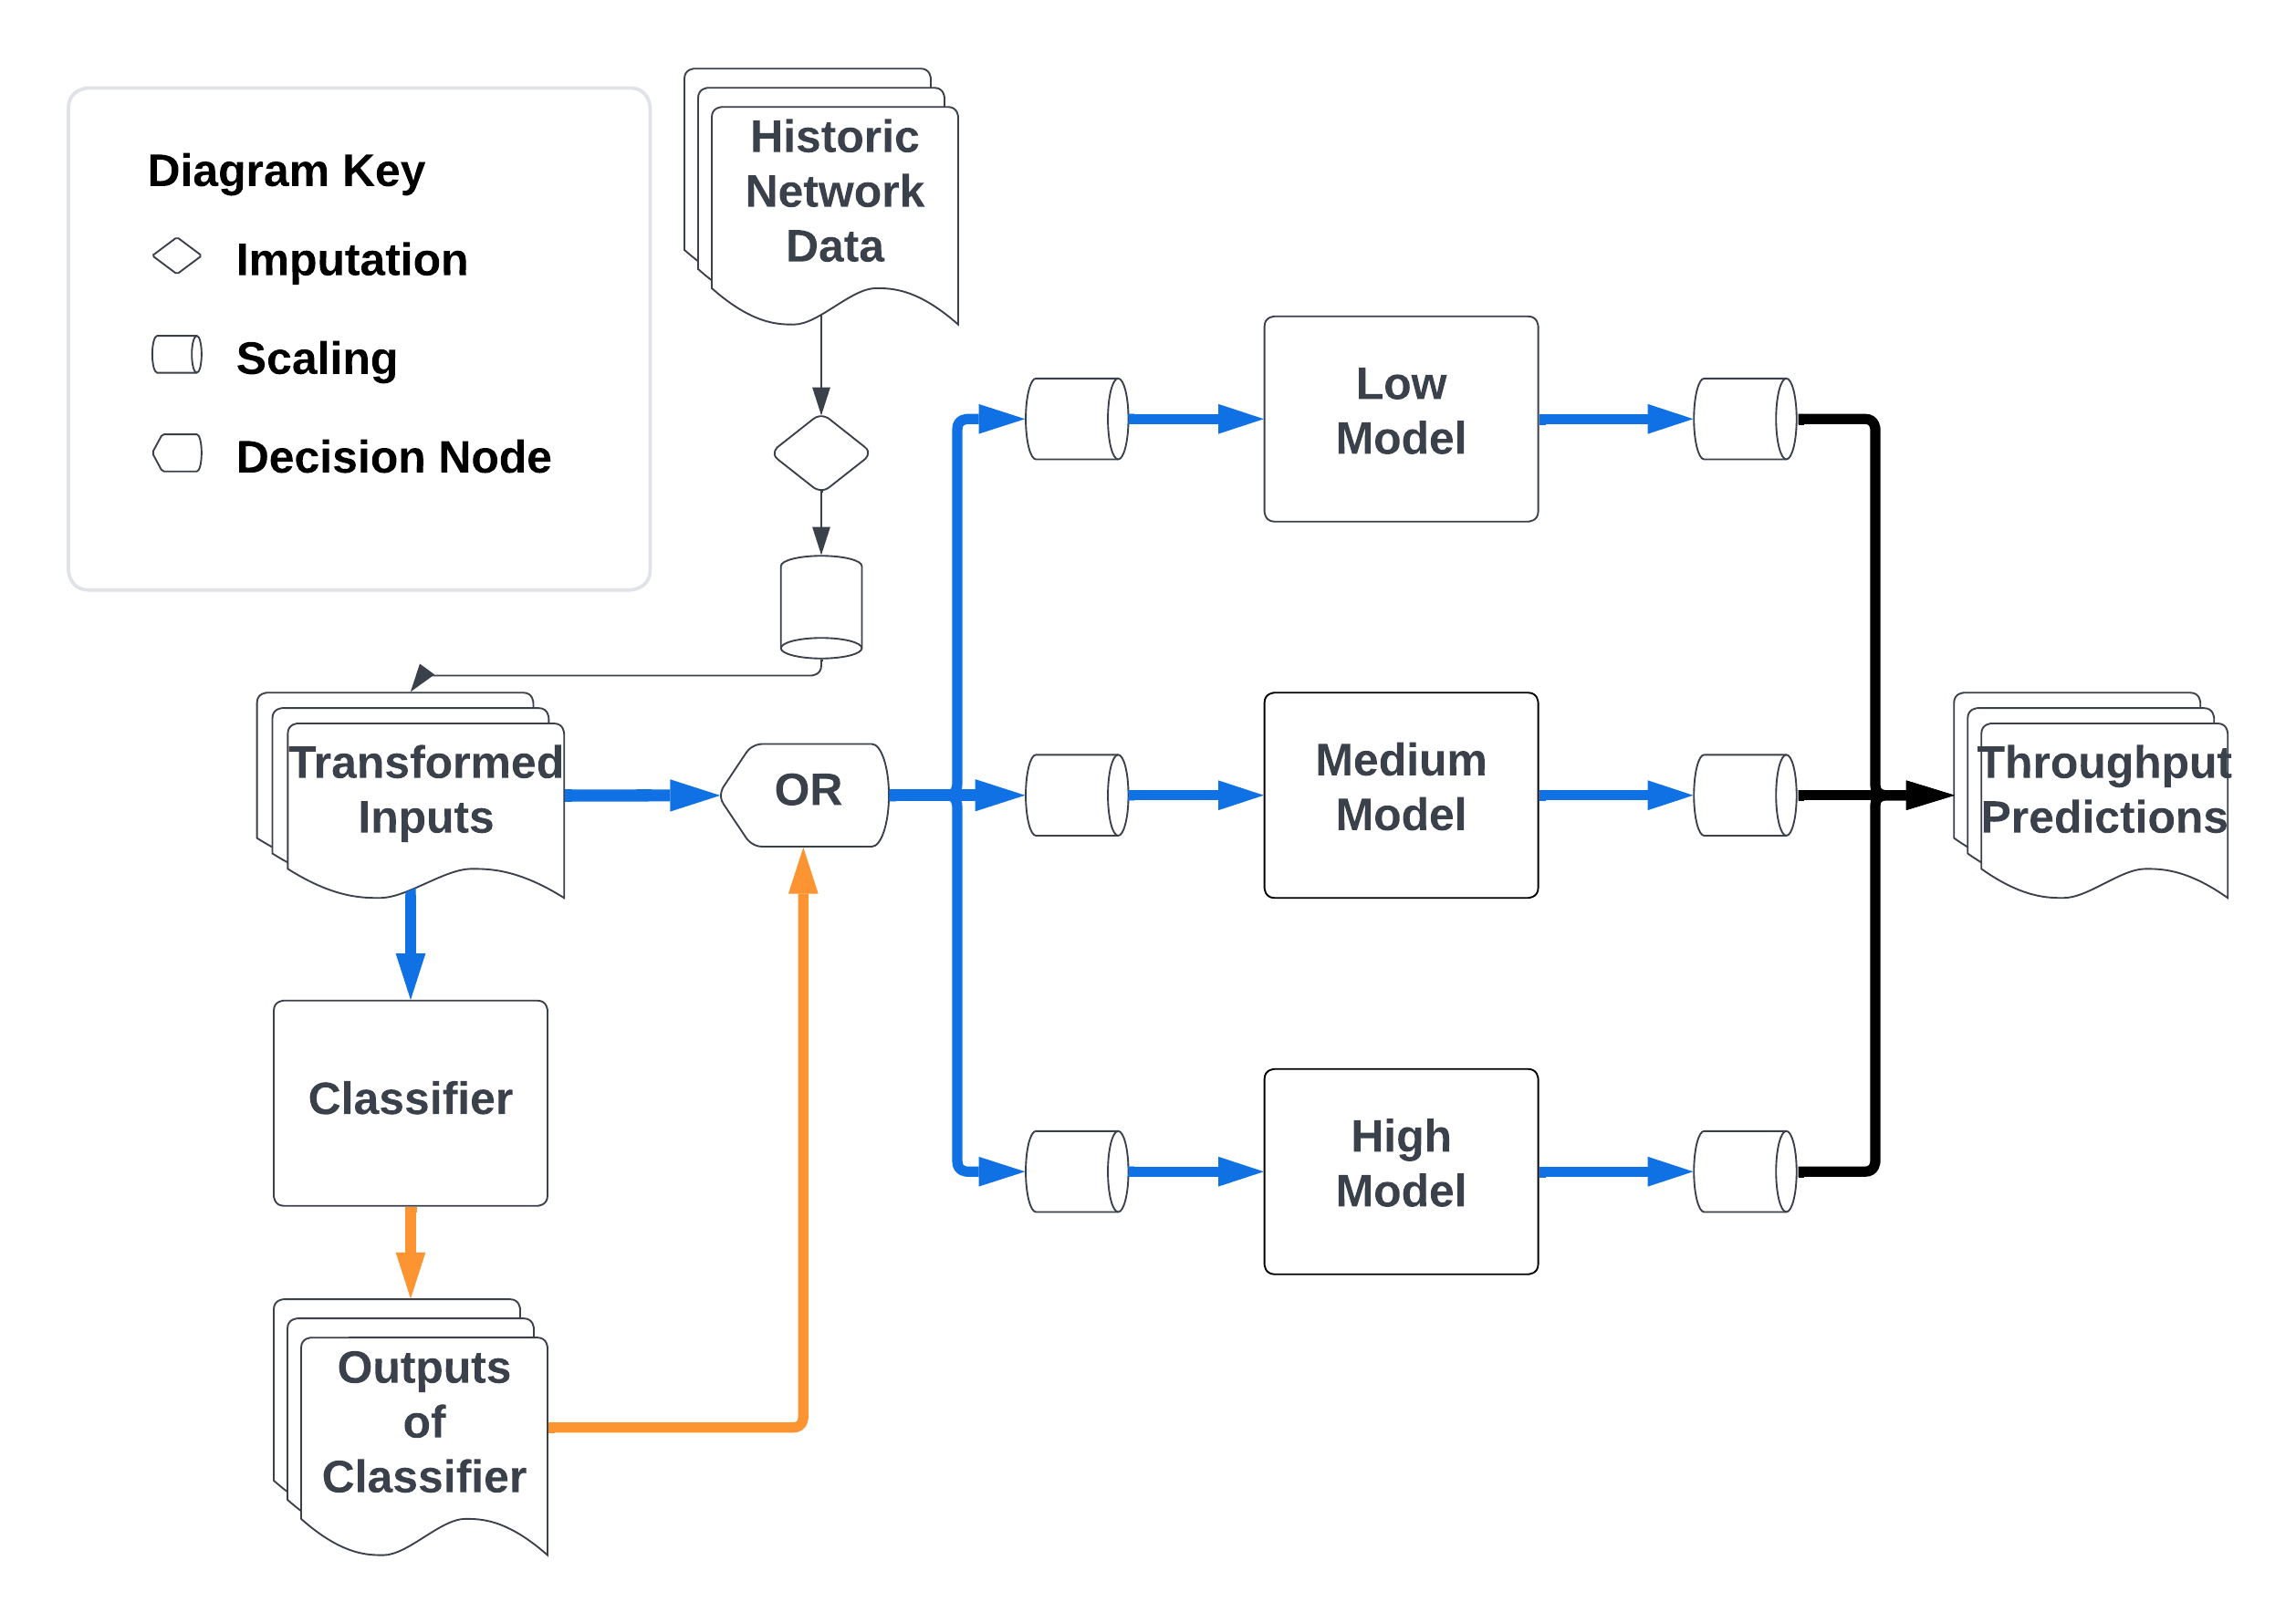
\includegraphics[scale=0.15]{Multistage One.png}
\label{fig:multistage_one}
\caption{Multistage One model.}
\end{figure}

The multistage throughput predictor herein referred to by "multistage one" uses a classifier to predict the most likely throughput class of the horizon for a given history sequence. As previously discussed, three classes are considered, high, medium and low, which describe the group the horizon throughput based on sub-ranges. Refer back to section \ref{sec:bounds} for a detailed description on the construction of these classes from the dataset. Based on the classifier's decision, the input is passed to one of the three regression models, each trained exclusively on examples of sequences of their respective class. As only one model is chosen, performance of this architecture is heavily dependent on correct classification of the horizon throughput scenario by the classifier. Misclassification of an input sequence will lead to the wrong regression model being chosen for throughput prediction negating the advantage of the multistage approach vs a single model entirely. Figure \ref{fig:multistage_one} shows the higher level design of the multistage one model.

\section{Multistage All}
\begin{figure}[h]
\centering
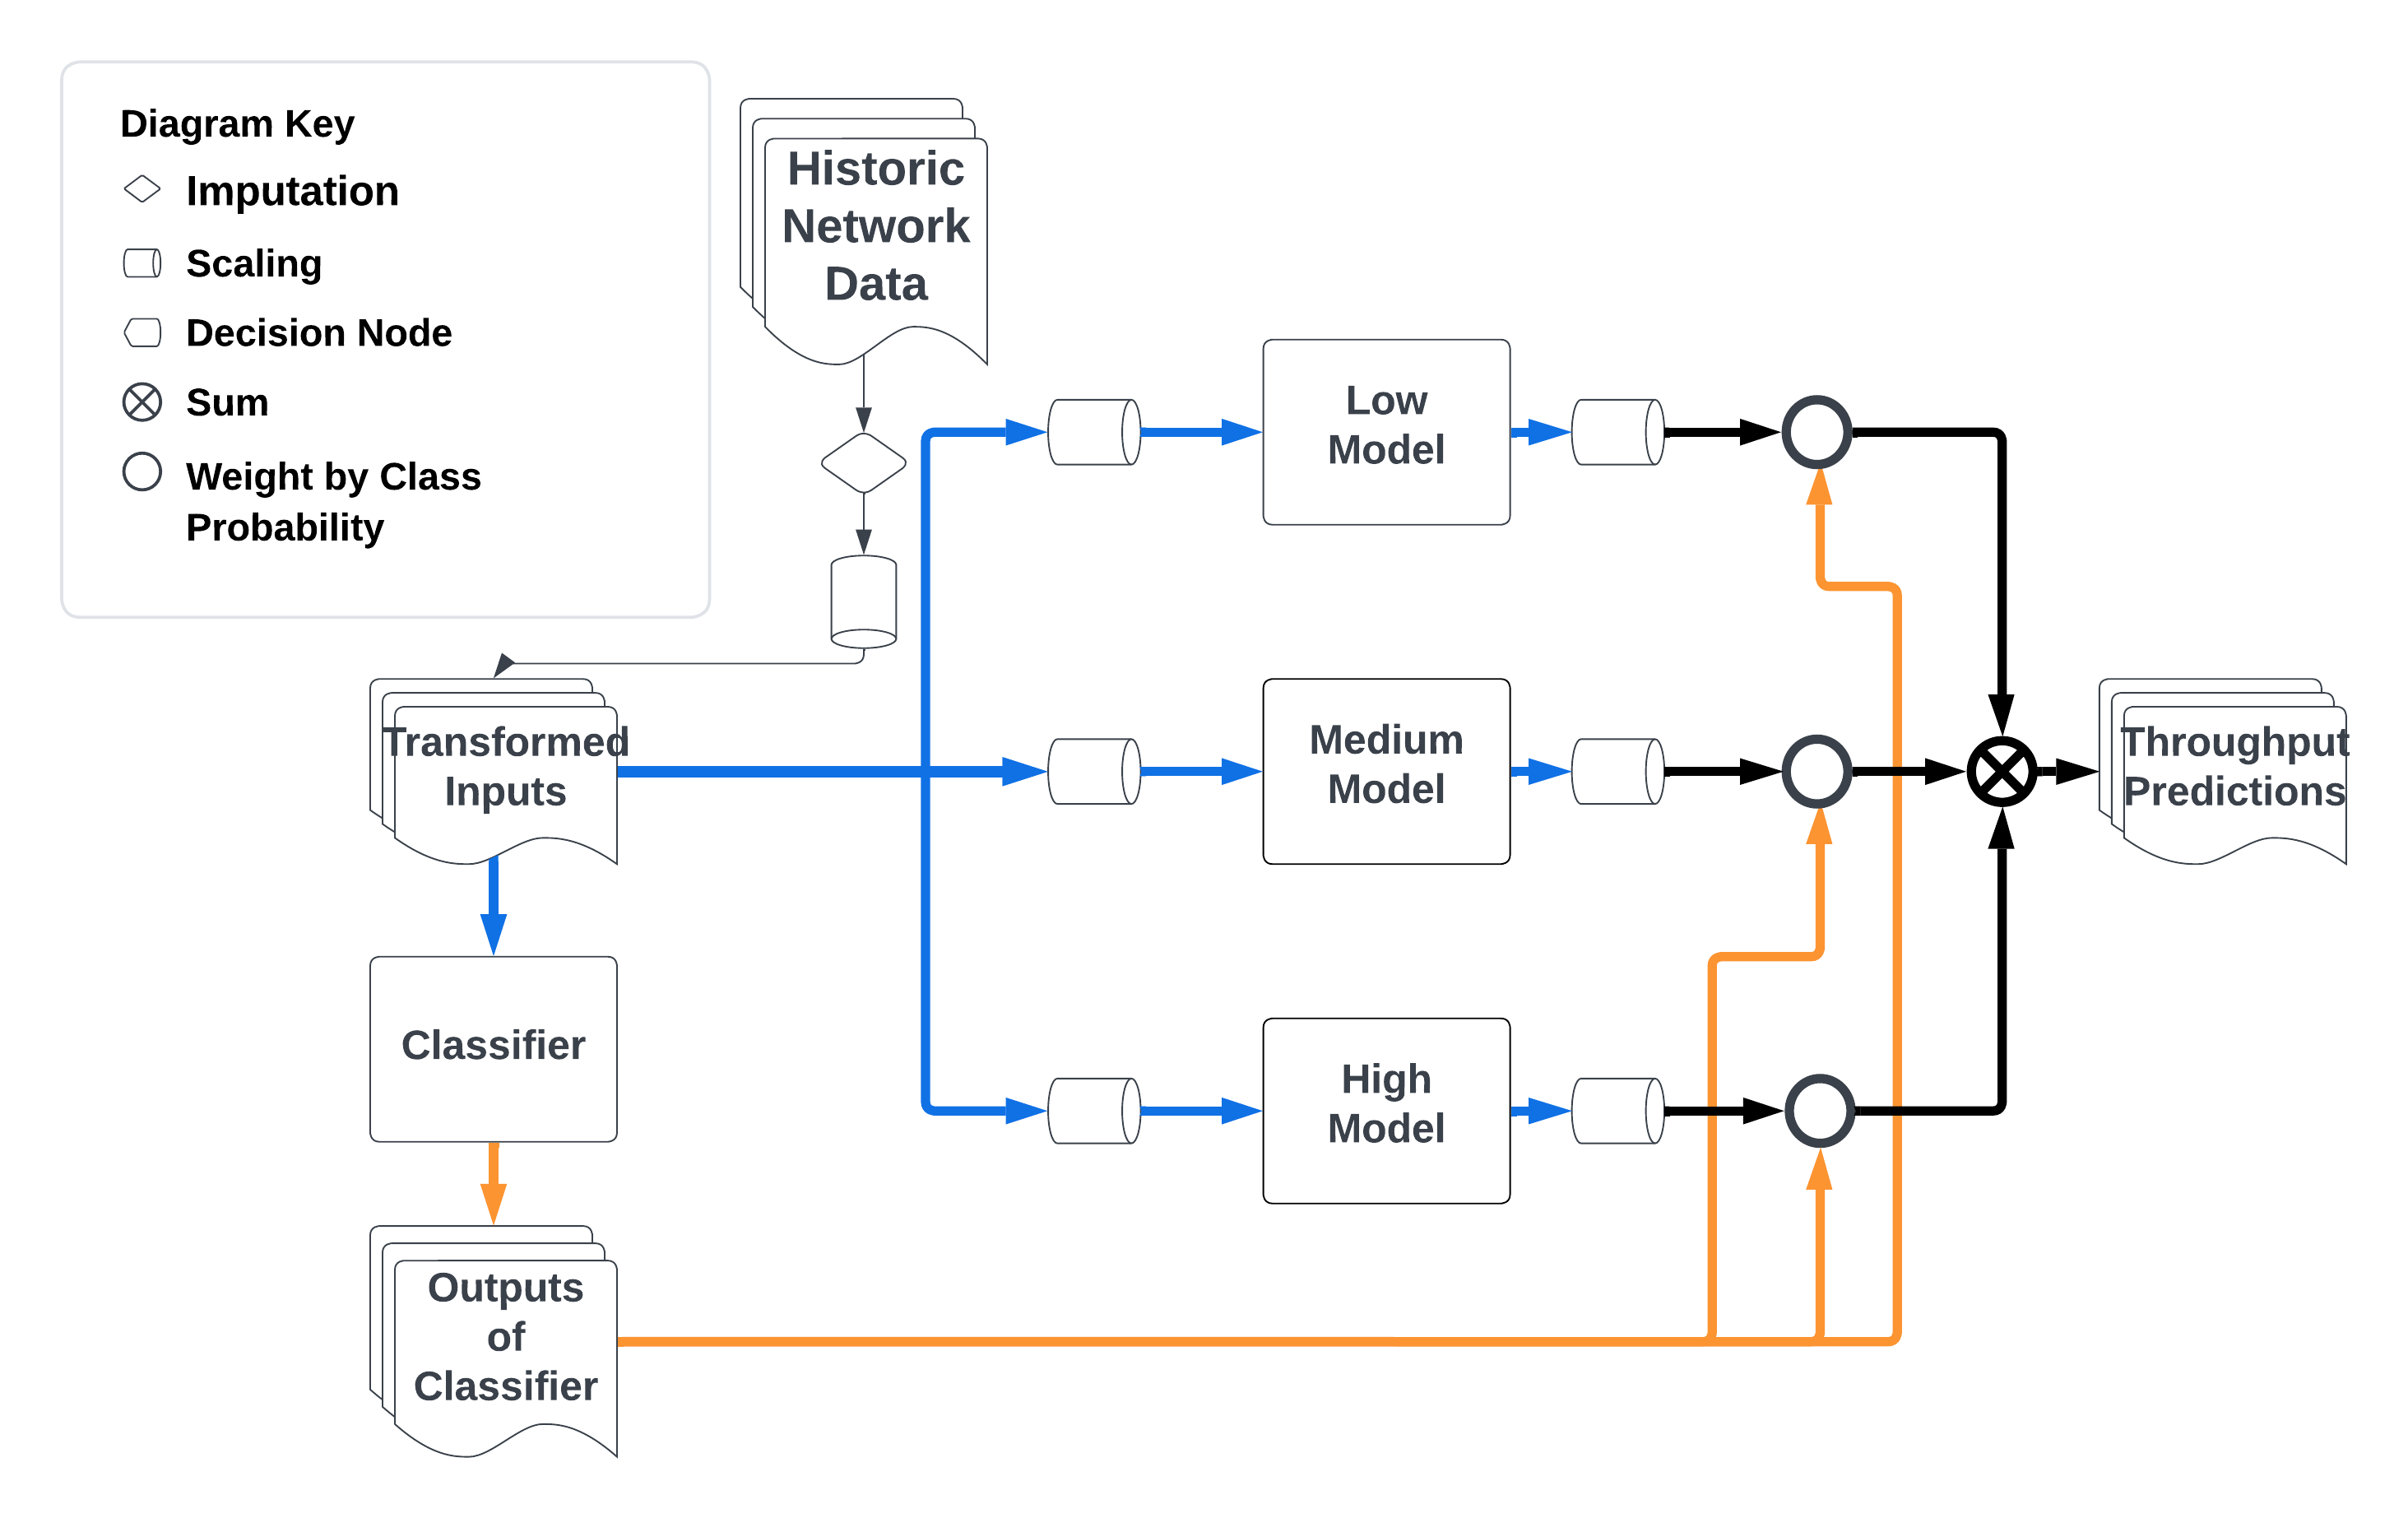
\includegraphics[scale=0.15]{Multistage All.png}
\label{fig:multistage_all}
\caption{Multistage All model.}
\end{figure}

The multistage throughput predictor herein referred to by "multistage all" uses a classifier to predict the probability of each of the classes of the horizon for a given history sequence. Unlike the multistage one model, the input sequence is then passed to all three regression models. The outputs of the regression models are then weighted by the class probability vector from the classifier and summed to create the final prediction. This is essentially an ensemble model. Ensemble models are known to perform better than using a single model \cite{https://doi.org/10.1002/widm.1249}. This model should perform better in situations where the classifier made less definite predictions on the input sequence's class. In theory, sequences on the border of two classes are better accommodated for by this model compared to the multistage one model. Figure \ref{fig:multistage_all} shows the higher level design of the multistage all model.

\section{Testing Framework}
To properly test the multistage approaches we first had to prove the rational to construct the multistage models based on the division of the range of DL\_bitrate. To do this we first test the individual regression models on their respective test sets and compare this to the baseline model's performance on the same test set. This shows that a model trained on a restricted range will be better at predicting values within that range. We then compare the performance of the multistage one, multistage all and baseline model on the complete test set. The complete test set is the baseline model's test set or the sum of the low, medium and high model's test sets. This shows actual performance of the multistage approaches as test sequences will be passed through the entire multistage frameworks for inference. We then considered the multistage models performance on the low and medium test sets in particular vs the baselines performance to identify in where difference in overall performance stemmed from. Results were calculated on the actual scale of the data in order to improve the understandability.

The following metrics were considered in the comparison:

- Mean Squared Error (MSE)\\
- Mean Absolute Error (MAE)\\
- Mean Absolute Percent Error (MAPE)\\
- Residual boxplots \\ 
- Absolute Percent Error boxplots \\

Relative error metrics such as MAPE are the most important in this application as they take into account that errors in lower throughput situations are more critical than errors in high throughput situations. I.e. A difference of 2Mbps in the prediction vs the true throughput when the predicted value is 152Mbps and the true value is 150Mbps is far less important than a difference in 2Mbps when the predicted throughput is 3Mbps and the true throughput is 1Mbps.

All tests were run on the same system. Specs are as follows: \\

- Cpu : Ryzen 5 1600 (6 cores / 12 threads) \@ 3.6Ghz
- GPU : Gtx 1050ti
- Ram : 32GB cl 3200 